\documentclass[a4paper,article,14pt]{extarticle}

% Подключаем главный пакет со всем необходимым
\usepackage{spbudiploma}

% Пакеты по желанию (самые распространенные)
% Хитрые мат. символы
\usepackage{euscript}
% Таблицы
\usepackage{longtable}
\usepackage{makecell}
% Картинки (можно вставлять даже pdf)
\usepackage[pdftex]{graphicx}

\usepackage{amsthm,amssymb, amsmath}
\usepackage{textcomp}

\usepackage{minted} % для примеров кода (требует параметра -shell-escape)
\usemintedstyle{bw}


\begin{document}

% Титульник в файле titlepage.tex
\newgeometry{left=30mm, top=20mm, right=15mm, bottom=20mm, nohead, nofoot}
\begin{titlepage}
\begin{center}

\textbf{Санкт--Петербургский государственный университет}\\
\textbf{Факультет математики и компьютерных наук}


\vspace{35mm}

\textbf{\textit{\large Имя Отчество Фамилия}} \\[8mm]
% Название
\textbf{\large Выпускная квалификационная работа}\\[3mm]
\textbf{\textit{\large Тема работы: довольно длинное название\\строки на две минимум}}

\vspace{20mm}
Уровень образования: бакалавриат\\
Направление 01.03.02 «Прикладная математика и информатика»\\
Основная образовательная программа СВ.5005.2018
«Прикладная математика, фундаментальная информатика и программирование»\\
Профиль «Современное программирование»\\[25mm]


% Научный руководитель, рецензент
\begin{flushright}
\begin{minipage}[t]{0.65\textwidth}
{Научный руководитель:} \\
профессор, д.ф.-м.н. А.\,А.\,Выбегалло
\vspace{10mm}

{Рецензент:} \\
старший разработчик ООО <<Рога и копыта>>\\ А.\,И.\,Привалов
\end{minipage}
\end{flushright}

\vfill

{Санкт-Петербург}
\par{\the\year{} г.}
\end{center}
\end{titlepage}
\restoregeometry
\addtocounter{page}{1}


% Содержание
\tableofcontents
\pagebreak

\specialsection{Введение}

%\todo{Введение широко представляет предметную область работы, указывает на место работы в научном или технологическом контексте.}

%\todo{О чем можно сказать, наверное:  котлин, мультиплатформа, single code base, time to market, преимущества (время, деньги, ошибки, ...), разные платформы и их ограничения....}

Современный рынок разработки ИТ-продуктов чрезвычайно конкурентен. От скорости создания  минимального жизнеспособного продукта (MVP) может зависеть положение на этом рынке и пользовательский охват. В последнее время популярность набирают языки и инструменты, позволяющие создавать приложения из единой кодовой базы под множество целевых платформ: начиная от настольных компьютеров под управлением операционных систем Windows, Linux и Mac OS X, и заканчивая умными часами (watchOS) или умными телевизорами (tvOS). Такими, например, являются фреймворк Flutter, который написан на языке Dart, а также Kotlin Multiplatform, который является инструментом языка Kotlin. Оба этих инструмента относительно новые --- первые публичные версии стали доступны в 2017 году, --- и поэтому имеют недостаток в виде отсутствия большого набора готовых библиотек для разных нужд. Одним из недостатков подобных инструментов является также ограниченность доступной из общего кода функциональности, поскольку вся такая функциональность должна иметь реализацию на всех целевых платформах.

Примером такой функциональности является работа с файлами и файловыми системами. В частности, для Kotlin Multiplatform нет стандартного способа работы с файловыми хранилищами из общего кода, а значительным недостатком многих существующих решений является отсутствие поддержки браузерной платформы. Запрос от сообщества разработчиков на подобные решения подтверждается вопросами по этой теме на популярных интернет-площадках\cite{so-file-io-with-kotlin-multiplatform, so-read-write-file-in-kotlin-native-ios-side, reddit-multiplatform-file-io, reddit-kotlin-native-library-io, kotlinlang-multiplatform-file-interaction}. В данной работе изучается изложенная проблема и представляется решение в виде мультиплатформенной Kotlin-библиотеки, предоставляющее доступ к файловым хранилищам и поддерживающее в том числе браузерную платформу.

%В частности, при исполнении приложения в веб-браузере доступ к файловой системе компьютера запрещен, ввиду соображений безопасности. 

%\paragraph{Актуальность работы.} 

\vspace*{-0.6em}
\paragraph{Структура работы.} В разделе~\ref{overview} осуществлен разбор предметной области и альтернативных решений данной проблемы. В разделе~\ref{solution} представлена реализованная мультиплатформенная библиотека. В разделе~\ref{solution-details} рассказывается о технических деталях её реализации. В разделе~\ref{usage-examples} представлены примеры приложений, созданных на базе данной библиотеки.


\specialsection{Постановка задачи}

Цель работы состоит в разработке мультиплатформенной библиотеки на языке программирования Kotlin, позволяющей разработчику описывать логику работы с различными файловыми хранилищами в общем модуле мультиплатформенного проекта. Библиотека должна предоставлять интерфейс (виртуальной) файловой системы с иерархической структурой папок и файлов и позволять записывать и читать файлы как массивы байт. Библиотека должна быть достаточно гибкой, чтобы разработчик мог самостоятельно дополнить её функциональность (например, поддержать на базе библиотеки новое облачное хранилище), а также иметь возможность расширения на уровне предоставляемых интерфейсов, когда от целевых хранилищ требуется поддержка особых возможностей (например, наличие у файлов атрибутов прав на чтение/запись). 

От конечного продукта ожидается как минимум:
\begin{itemize}
    \item поддержка трех платформ: JVM (для приложений, работающих в среде операционных систем Windows, Linux, и т.д.), JS (браузерные приложения), Android (мобильные приложения);
    \item поддержка как минимум одного облачного хранилища, доступного со всех поддерживаемых платформ.
\end{itemize}

% Предлагается следующий план выполнения задачи:
% \begin{enumerate}
%     \item разобраться в предметной области, выделить ключевые проблемы;
%     \item провести исследование существующих решений с открытым исходным кодом;
%     \item с учетом полученных данных разработать архитектуру библиотеки;
%     \item реализовать библиотеку, а также поддержку нескольких хранилищ для примера;
%     \item написать относительно простое мультиплатформенное приложение на базе библиотеки, иллюстирующее преимущества и недостатки получившегося решения;
%     \item провести анализ получившегося продукта.
% \end{enumerate}



\section{Обзорный раздел по предметной области}

\subsection{Использование формул}



Ненумерованная формула:

\begin{equation}
    \begin{pmatrix} \dot{\varphi}\\ \dot{\theta} \\ \dot{\psi} \end{pmatrix}
    = \begin{pmatrix}
        cos(\theta)cos(\psi) & -sin(\psi) & 0 \\
        cos(\theta)sin(\psi) & cos(\psi)  & 0 \\
        -sin(\theta)         & 0         &  1
    \end{pmatrix}^{-1}
    \begin{pmatrix} \omega_x\\ \omega_y \\ \omega_z \end{pmatrix}.
\end{equation}

Нумерованная формула:

\begin{equation}
    i^2 = -1.
    \label{eq:my_ref}
\end{equation}

Тест ссылки на формулу \ref{eq:my_ref}.

\subsection{Вставка рисунков}

\begin{figure}[ht]
\begin{center}
\scalebox{0.4}{
   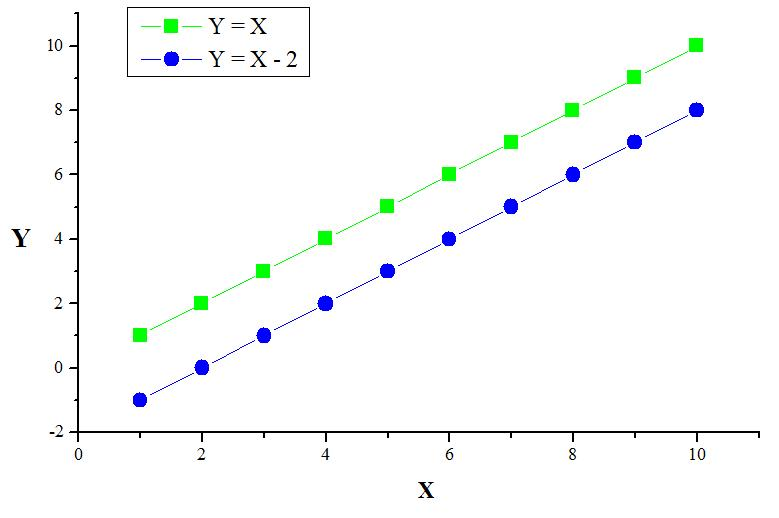
\includegraphics{images/graph.jpg}
}

\caption{
\label{graph-fig}
     Линейные функции.}
\end {center}
\end {figure}
Ссылаемся на график~\ref{graph-fig}.

\subsection{Ссылки на источники}

Ссылки на источники: \cite{voc}, \cite{vo2}, \cite{ij-sdk}.

\subsection{Оформление фрагментов кода}

В работах иногда приводят фрагменты кода:

\begin{minted}{kotlin}
fun main() {
    val name = "stranger"
    println("Hi, $name!")
    print("Current count:")
    for (i in 0..10) {
        print(" $i")
    }
}
\end{minted}


\subsection{Оформление таблиц}


\begin{table}[ht]
\begin{center}
\begin{tabular}{lccc}
    Имя & Работа 1 & Работа 2 & Итог \\
\hline
    Алиса & 8.0 & 9.0 & 8.5 \\
    Боб & 9.0 & 9.8 & 9.4 \\
    Чак & 9.1 & 9.3 & 9.2 \\
\end{tabular}
\caption{
\label{table-smth}
     Сравнение результатов.}
\end {center}
\end {table}

Ссылаемся на таблицу~\ref{table-smth}.




\section{Основной раздел}

\subsection{Подраздел}
\subsection{Подраздел}
\subsection{Подраздел}

\section{Основной раздел}

\subsection{Подраздел}
\subsection{Подраздел}
\subsection{Подраздел}

% !TEX root = ../main.tex


\section{Заключительный раздел с основными результатами}

\subsection{Подраздел}



\subsection{Подраздел}



\specialsection{Заключение}

Заключение должно подводить итоги работы и содержать информацию о полученных в рамках работы результатах.



% Аргумент {1} ниже включает переопределенный стиль с выравниванием слева
\begin{thebibliography}{1}
\bibitem{voc} D.W. Griffin, J.S.Lim. Multiband excitation vocoder. IEEE ASSP-36 (8), 1988, pp. 1223-1235.
\bibitem{vo2} A. Golovnev, A. S. Kulikov, I. Mihajlin. Families with Infants: Speeding Up Algorithms for NP-Hard Problems Using FFT., ACM Transactions on Algorithms, 12:3, 2016.
\bibitem{ij-sdk} IntelliJ Platform SDK. URL: \url{https://plugins.jetbrains.com/docs/intellij/welcome.html} (дата обр. 10.02.2022).
\end{thebibliography}
\end{document}